% Section content template for individual Educative lessons
% This file contains the actual content for a specific section
% Generated from Educative API section content

% Section: Structural Design Patterns

% Section ID: 5770496058851328
% Section Slug: structural-design-patterns
% Generated: 2025-12-11T06:16:21.659509

\subsection{Introduction to structural patterns}\label{introduction-to-structural-patterns}
\\
In this lesson, we will discuss structural design patterns. As the name implies, these patterns are concerned with object relationships and the structure of classes or objects. They help to add new functionality without having to modify the entire system. They ensure that if one part of a system changes, the whole system does not change with it. Let 's look at the most common structural patterns that are used in solving design problems.

\begin{figure}[htbp]
 \centering
 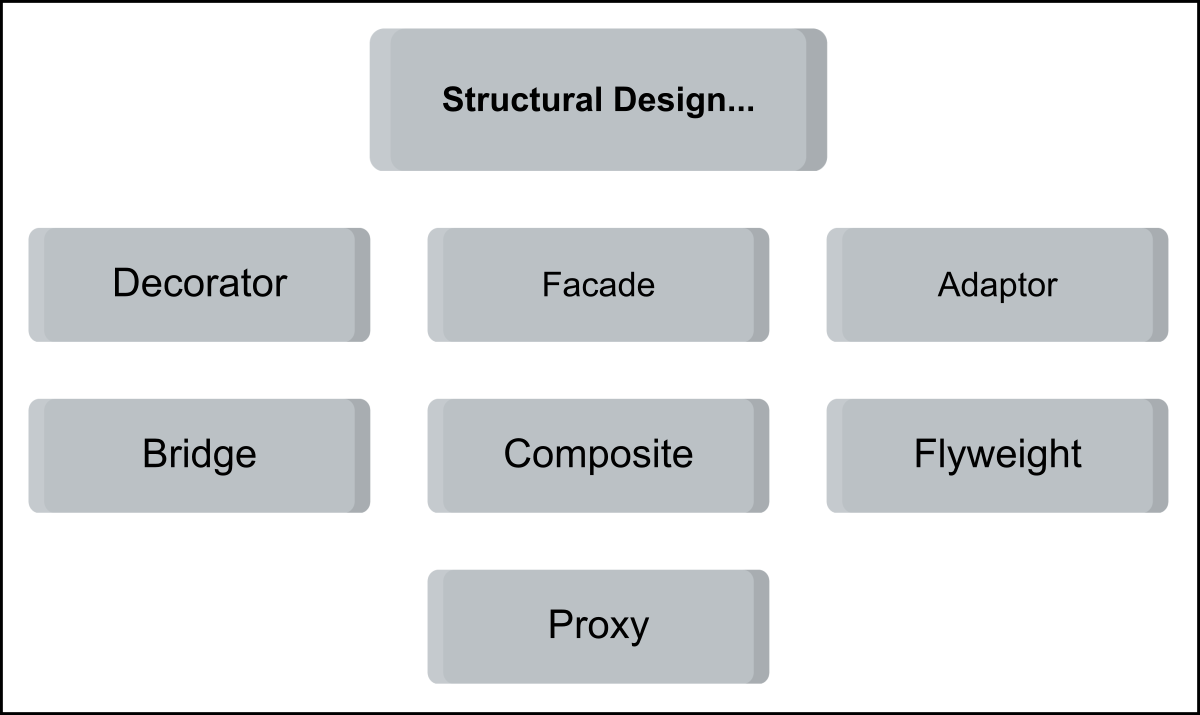
\includegraphics[width=0.5\textwidth]{Images/chapter_5/section_5770496058851328/5746954749607936.png}
 \caption{Structural design patterns}
\end{figure}

\subsection{Decorator pattern}\label{decorator-pattern}
\\
The \textbf{Decorator pattern} focuses on adding properties, functionalities, and behavior to existing classes dynamically. The additional decoration functionalities aren't considered essential enough to be a part of the original class definition since they can cause clutter. Hence, the Decorator pattern lets us modify the code without changing the original class.
\\
Unlike creational patterns, the Decorator pattern is a structural pattern that does not focus on object creation but rather on decoration. Hence , it doesn't rely on prototypal inheritance alone. It takes the object and keeps adding decoration to it. This makes the process more streamlined. Let's look at an example to understand this concept better.
\\
The illustration below shows that ice-cream toppings can be a part of the Decorator pattern for a plain vanilla cone.

\begin{figure}[htbp]
 \centering
 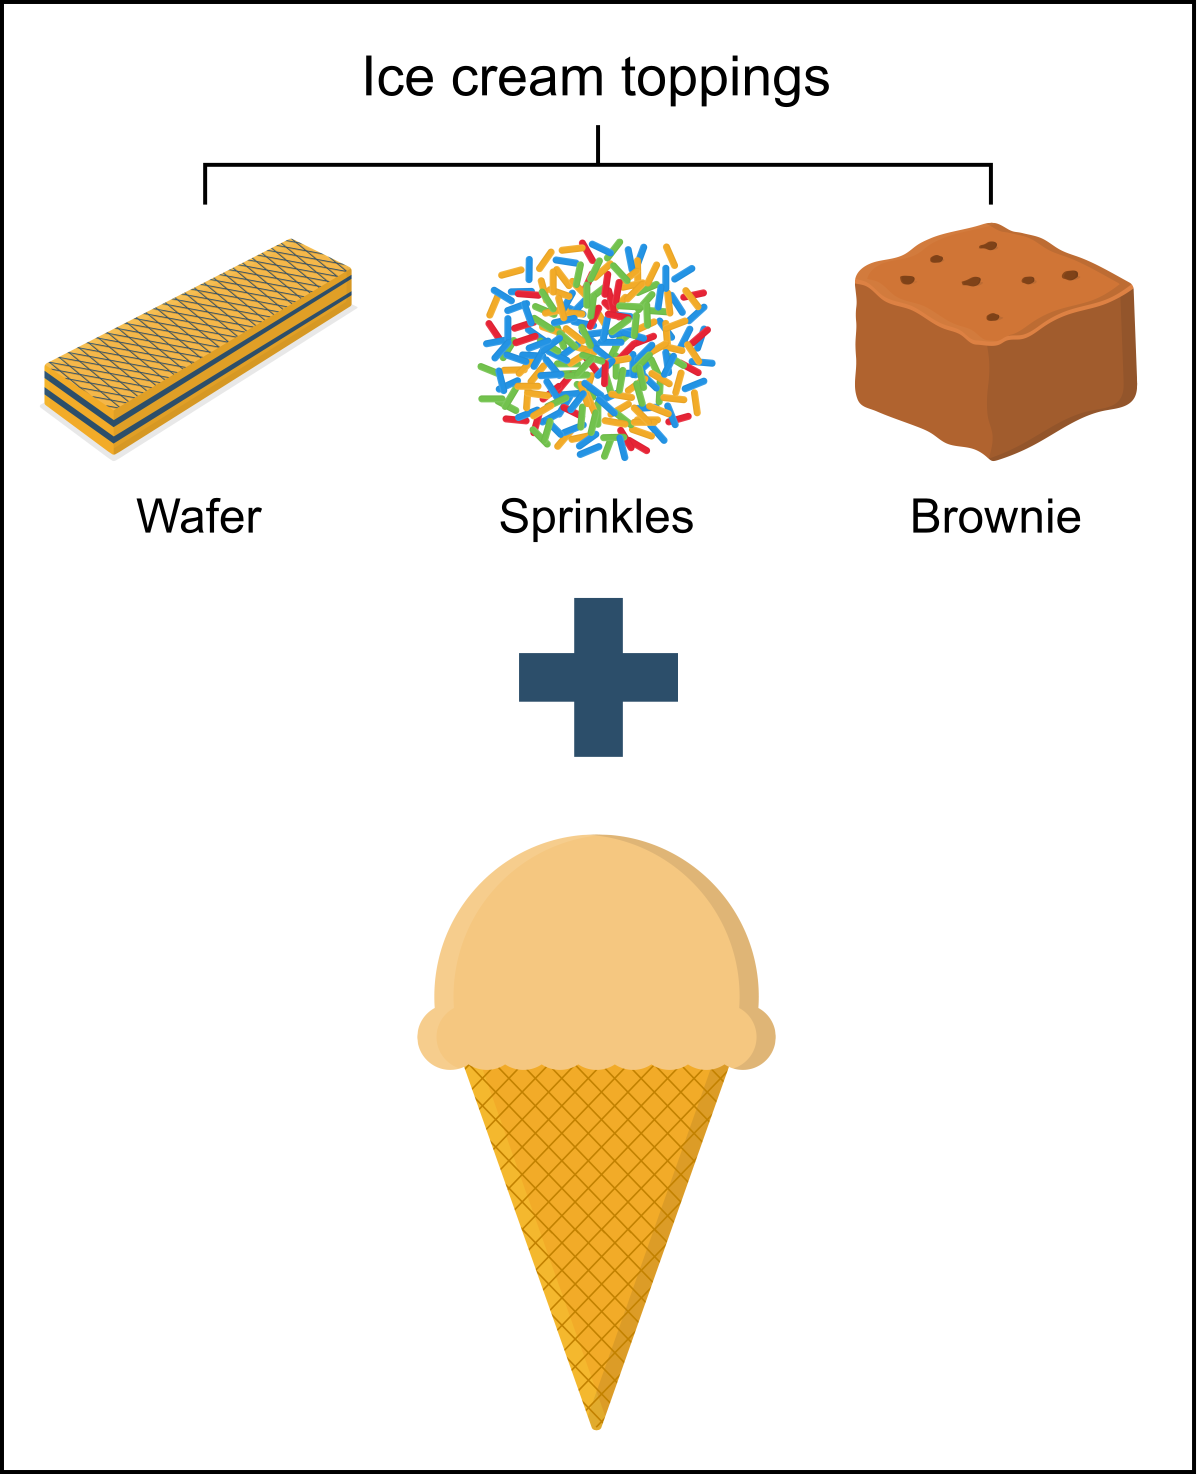
\includegraphics[width=0.25\textwidth]{Images/chapter_5/section_5770496058851328/5809023699124224.png}
 \caption{Ice-cream toppings can be implemented using the Decorator pattern}
\end{figure}

\subsection{Facade pattern}\label{facade-pattern}
\\
The word ``\textbf{facade}'' means a deceptive front or appearance. Following this definition, a \textbf{Facade pattern} provides a simpler interface that hides the complex functionalities of a system. The Facade pattern allows us to hide all the messy logic from the client and only display the clear and easy-to-use interface to them. This allows the client to interact with an API easily in a less error-prone way and without accessing the inner workings directly.

\subsection{Adapter pattern}\label{adapter-pattern}
\\
The \textbf{Adapter pattern} allows classes that have different interfaces (properties/methods of an object) to work together. It translates the interface for a class to make it compatible with another class.
\\
This pattern is useful if an API is modified or new implementations are added to it. In this case, if the other parts of a system are still using the old API, the Adapter pattern will translate the interface so that the two can work together. The illustration below demonstrates the use of the Adapter pattern.

\begin{figure}[htbp]
 \centering
 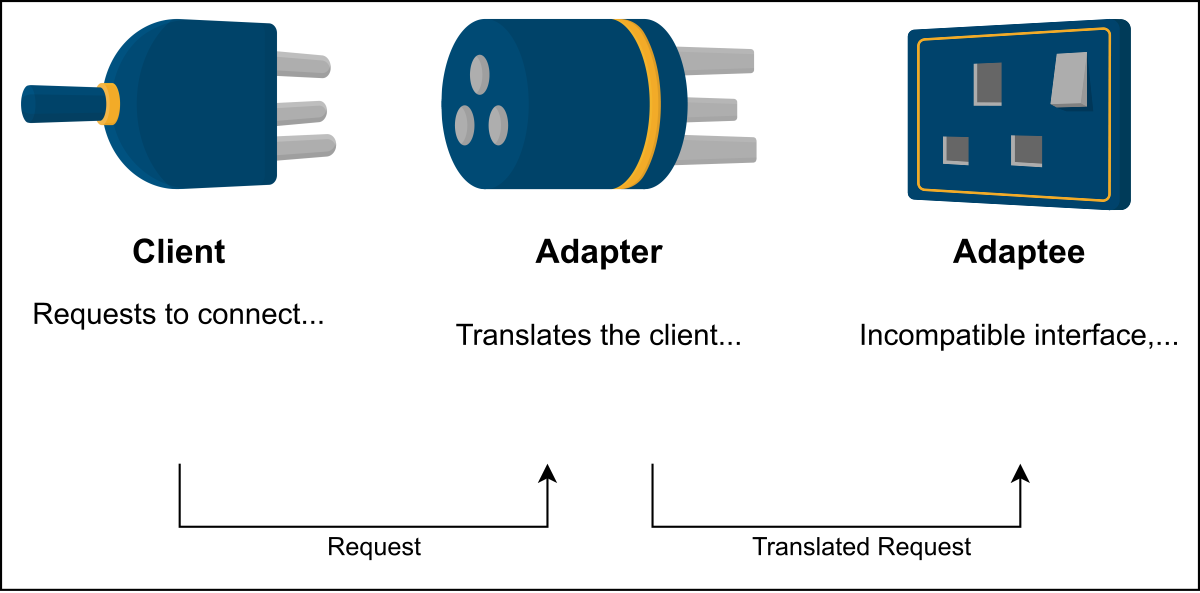
\includegraphics[width=0.5\textwidth]{Images/chapter_5/section_5770496058851328/5123571346309120.png}
 \caption{Concept for the Adapter pattern}
\end{figure}

\subsection{Bridge pattern}\label{bridge-pattern}
\\
The \textbf{Bridge pattern} allows separate components with separate interfaces to work together. It keeps an object's interface separate from its implementation, allowing the two to vary independently.
\\
An example is controlling an air conditioner with a remote. The air conditioners can be of different types and each of them is controlled by a different remote. The remotes can vary, that is, a new one with better features can be introduced, but that won't make any changes to the air conditioner classes. The same goes the other way round. The Bridge pattern allows input and output devices to work together but vary independently.

\subsection{Composite pattern}\label{composite-pattern}
\\
The \textbf{Composite pattern} is used to structure objects in a tree-like hierarchy. Here, each node of the tree can be composed of either child node(s) or be a leaf (no children objects). This pattern allows the client to work with these components uniformly, that is, a single object can be treated exactly how a group of objects is treated.
\\
This pattern allows the formation of a deeply-nested structure. If a leaf object receives the request sent by the client, it will handle it. However, if the recipient is composed of children, the request is forwarded to the child components.
\\
A Composite pattern consists of the following:

\begin{itemize}
\item
\textbf{Component:} An abstract class that contains methods such as \texttt{add}, \texttt{remove}, and \texttt{get} that are used in managing the children. The component can be a leaf object or composite.
\item
\textbf{Composite:} This is the subclass that implements a component. It is composed of other components (children).
\item
\textbf{Leaf:} This is the subclass that implements a component. It does not have children.
\end{itemize}
\\
We can visualize this in the diagram below:

\begin{figure}[htbp]
 \centering
 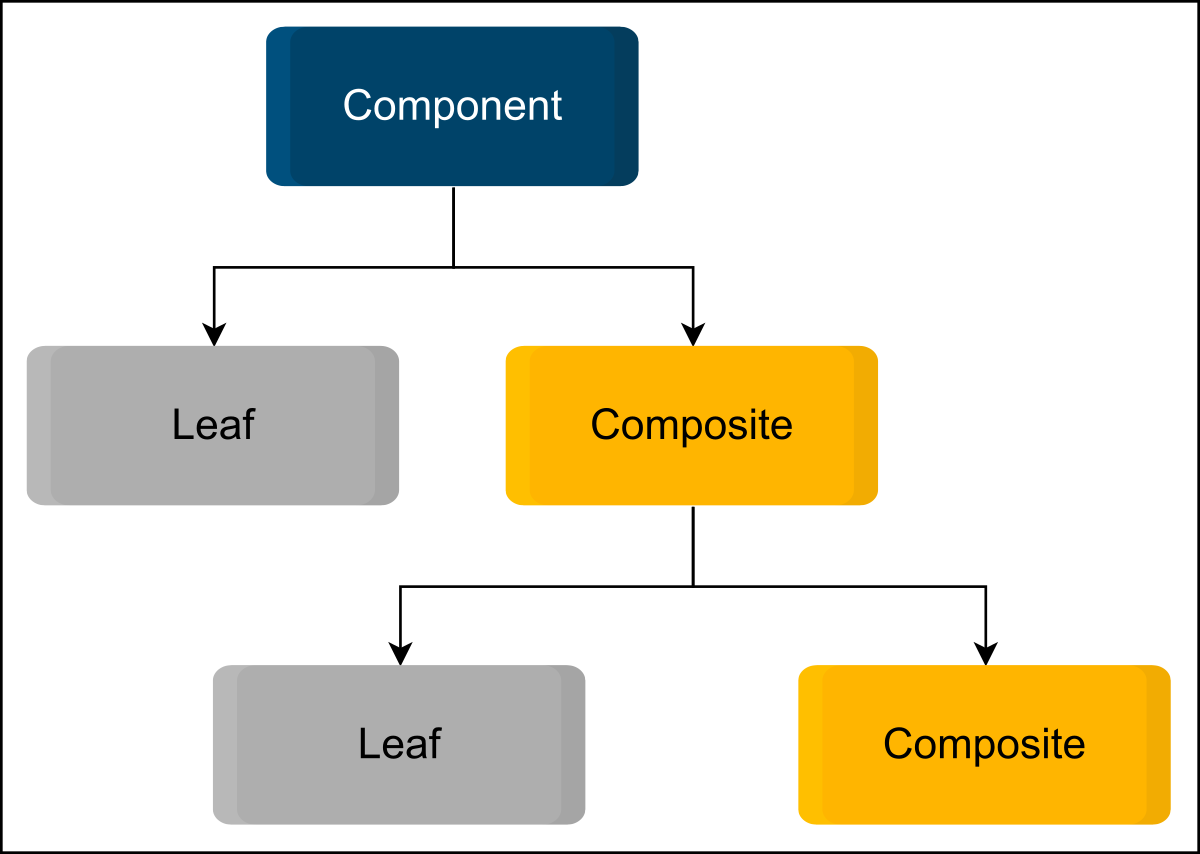
\includegraphics[width=0.25\textwidth]{Images/chapter_5/section_5770496058851328/6466721710080000.png}
 \caption{Concept for the Composite pattern}
\end{figure}

\subsection{Flyweight pattern}\label{flyweight-pattern}
\\
The \textbf{Flyweight pattern} focuses on how related objects share data. It helps prevent repetitive code and increases efficiency when it comes to data sharing as well as conserving memory.
\\
This pattern takes the common data structures/objects that are used by a lot of objects and stores them in an external object (flyweight) for sharing. We can say that it is used for caching purposes. So , the same data does not need to have separate copies for each object, instead, it is shared amongst all.
\\
A flyweight is an independent object that can be used in multiple contexts simultaneously. It cannot be distinguished from the instances of objects that are not sharable. A flyweight object can consist of two states:

\begin{itemize}
\item
\textbf{Intrinsic:} This state is stored in the flyweight. It contains the information required by the internal methods of objects. It is independent of the context of the flyweight and is sharable with other objects.
\item
\textbf{Extrinsic:} This state depends on the context of the flyweight and it cannot be shared. Normally, the client objects pass the extrinsic state to the flyweight object when needed.
\end{itemize}
\\
Let\textquotesingle s see a visual depiction of the Flyweight pattern:

\begin{figure}[htbp]
 \centering
 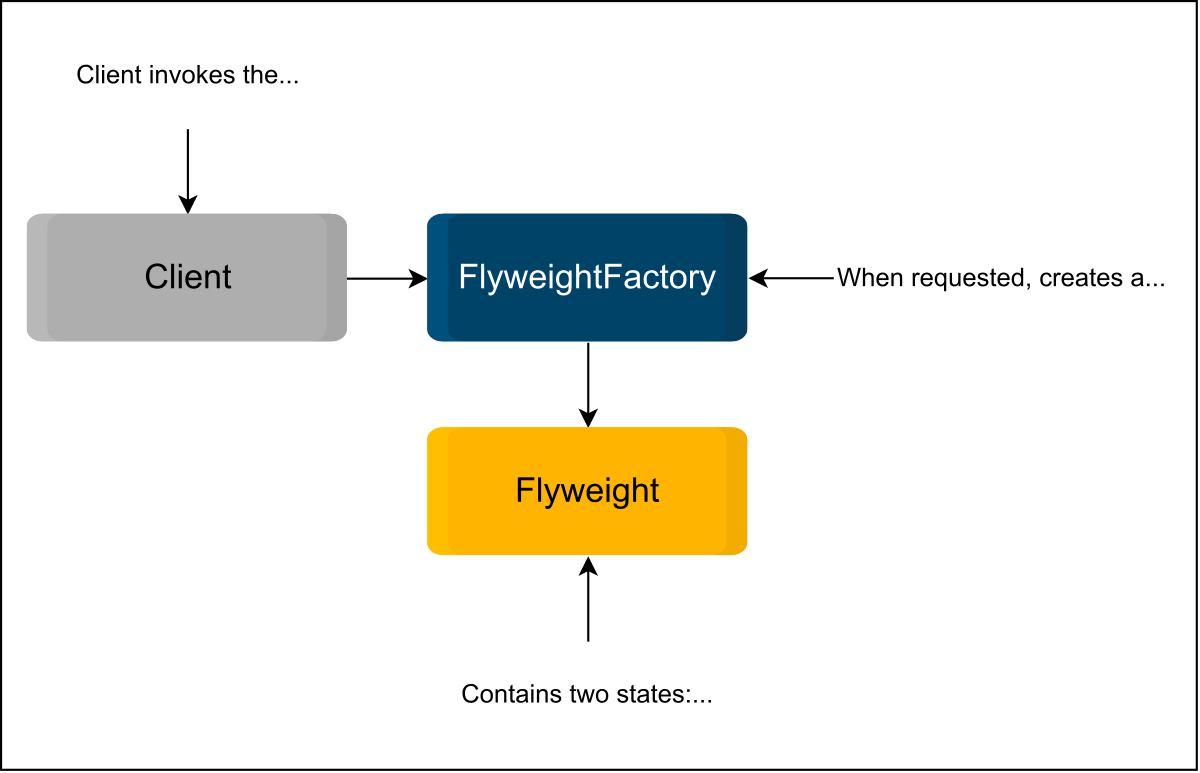
\includegraphics[width=0.5\textwidth]{Images/chapter_5/section_5770496058851328/6675121269112832.png}
 \caption{Concept for the Flyweight pattern}
\end{figure}

\subsection{Proxy pattern}\label{proxy-pattern}
\\
As the name implies, the \textbf{Proxy pattern} is a structural pattern that creates a proxy object. It acts as a placeholder for another object, controlling access to it.
\\
Usually, an object has an interface with several properties/methods that a client can access. However, an object might not be able to deal with the clients' requests alone due to heavy load or constraints such as dependency on a remote source that might cause delays (e.g., network requests). In these situations, adding a proxy helps in dividing the load with the target object.
\\
The proxy object looks exactly like the target object. A client might not even know that they are accessing the proxy object instead of the target object. The proxy handles the requests from the clients and forwards them to the target object, preventing undue pressure on the target.

\subsection{When to use structural patterns?}\label{when-to-use-structural-patterns}
\\
Let\textquotesingle s see when we can use the structural patterns discussed above:

\begin{table}[htbp]
\centering
\small
\adjustbox{max width=\textwidth}{
\begin{tabular}{|p{0.249\textwidth}|p{0.701\textwidth}|}
\hline
\textbf{Structural Design Patterns} & \textbf{When to Use} \\
\hline
\hline
\hfill\break Decorator \hfill\break & \begin{itemize} \tightlist \item To modify or extend the functionality of an object without changing its base code. \item To implement additional functionalities of similar objects instead of reusing the same code. \end{itemize} \\
\hline
\hfill\break Facade \hfill\break & \begin{itemize} \tightlist \item To simplify a client's interaction with a system by hiding the underlying complex code. \item To interact with the methods present in a library without knowing the processing that happens in the background. \end{itemize} \\
\hline
\hfill\break Adapter & \begin{itemize} \tightlist \item To enable old APIs to work with new refactored ones. \item To allow an object to cooperate with a class that has an incompatible interface. \item To reuse the existing functionality of classes. \end{itemize} \\
\hline
\hfill\break Bridge & \begin{itemize} \tightlist \item To extend a class in several independent dimensions. \item To change the implementation at run time. \item To share the implementation between objects. \end{itemize} \\
\hline
\hfill\break Composite & \begin{itemize} \tightlist \item To allow the reuse of objects without worrying about their compatibility. \item To develop a scalable application that uses plenty of objects. \item To create a tree-like hierarchy of objects. \end{itemize} \\
\hline
\hfill\break Flyweight \hfill\break & \begin{itemize} \tightlist \item To share a list of immutable strings across the application. \item To prevent load time as it allows caching. \end{itemize} \\
\hline
Proxy & \begin{itemize} \tightlist \item To reduce the workload on the target object. \end{itemize} \\
\hline
\end{tabular}
}
\end{table}

Next, let's look at the behavioral design patterns used in the object-oriented design.

% End of section content